%% chapter-1: 绪论部分
%% 介绍本研究课题的学术背景及理论与实际意义,国内外文献综述,
%% 本研究课题的来源及主要研究内容。
%重新设置headings
\fancypagestyle{headings}{
    \fancyhf{}
    \fancyfoot[C]{\songti\xiaowu 第 \thepage 页}
    \fancyhead[L]{\songti\xiaowu 上海工程技术大学硕士学位论文}
    \fancyhead[R]{\songti\xiaowu 第\zhnum{chapter} 章 \quad 绪\quad 论}
}
\pagestyle{headings}
\chapter{绪\quad 论}
\section{算法框架}

这里举例一个在文章当中插入的一个算法框架
\begin{center}
    \begin{minipage}{0.8\textwidth}
        \begin{algorithm}[H]%[!htp]
            \caption{算法的名字} %算法的名字
            {\bf 输入:} %算法的输入, \hspace*{0.02in}用来控制位置,同时利用 \\ 进行换行
            input parameters A, B, C\\
            {\bf 输出:} %算法的结果输出
            output result
        \begin{algorithmic}[1]
            \State some description 算法介绍 % \State 后写一般语句
            \For{condition} % For 语句,需要和EndFor对应
                \State ...
                \If{condition} % If 语句,需要和EndIf对应
                    \State ...
                \Else
                    \State ...
                \EndIf
            \EndFor
            \While{condition} % While语句,需要和EndWhile对应
                \State ...
            \EndWhile
            \State \Return result
            \end{algorithmic}
        \end{algorithm}
    \end{minipage}
    \label{algo:test_algoritm}
\end{center}

文章中标准的算法格式如算法\ref{algo:test_algoritm}所示,文章中以这种方式表示算法比较清晰可见。一般使用以上的算法框架可以清晰表示出算法的步骤程序。

\section{三线表画法}
前面已经说明了三线表的画法,这里再次举例一个三线表,如表\ref{tab2:heightweight}所示。

\begin{table}[!htp]
    \newcolumntype{L}{X}
    \newcolumntype{C}{>{\centering \arraybackslash}X}
    \newcolumntype{R}{>{\raggedright \arraybackslash}X}
    \centering
    \caption{某校学生升高体重样本}
    \label{tab2:heightweight}
    \begin{tabularx}{0.9\textwidth}{CCCC}
       \toprule[1.5pt]
        序号&年龄&身高&体重\\
        \midrule[0.75pt]
        1&14&156&42\\
        2&16&158&45\\
        3&14&162&48\\
        4&15&163&50\\
        \midrule[0.75pt]
        %\cmidrule{2-4}
        平均&15&159.75&46.25\\
        \bottomrule[1.5pt]
    \end{tabularx}
\end{table}
\section{多级标题示例}
一般共有三级标题,分为section,subsection,subsubsection三种标题,可以看到下面就是几个多级标题的例子。
\subsection{三级标题示例1}
文章章节引用的时候,可以设置一个标签label,然后用ref引用这个label。例如我在章节\ref{sec:my_section_label}处将对latex插图进行说明。
\subsection{三级标题示例2}
\section{latex插图处理}
\label{sec:my_section_label}

本章节介绍图片插入方法,一共有三种插入图片的方法,我在下面详细介绍。
\subsection{普通插图方法}
如图\ref{fig:my_pic1}所示,在这里我们插入了一个图片。其中可以自定义缩放比例以及图片的高度等等信息。
\begin{figure}[hbpt]
    \centering
    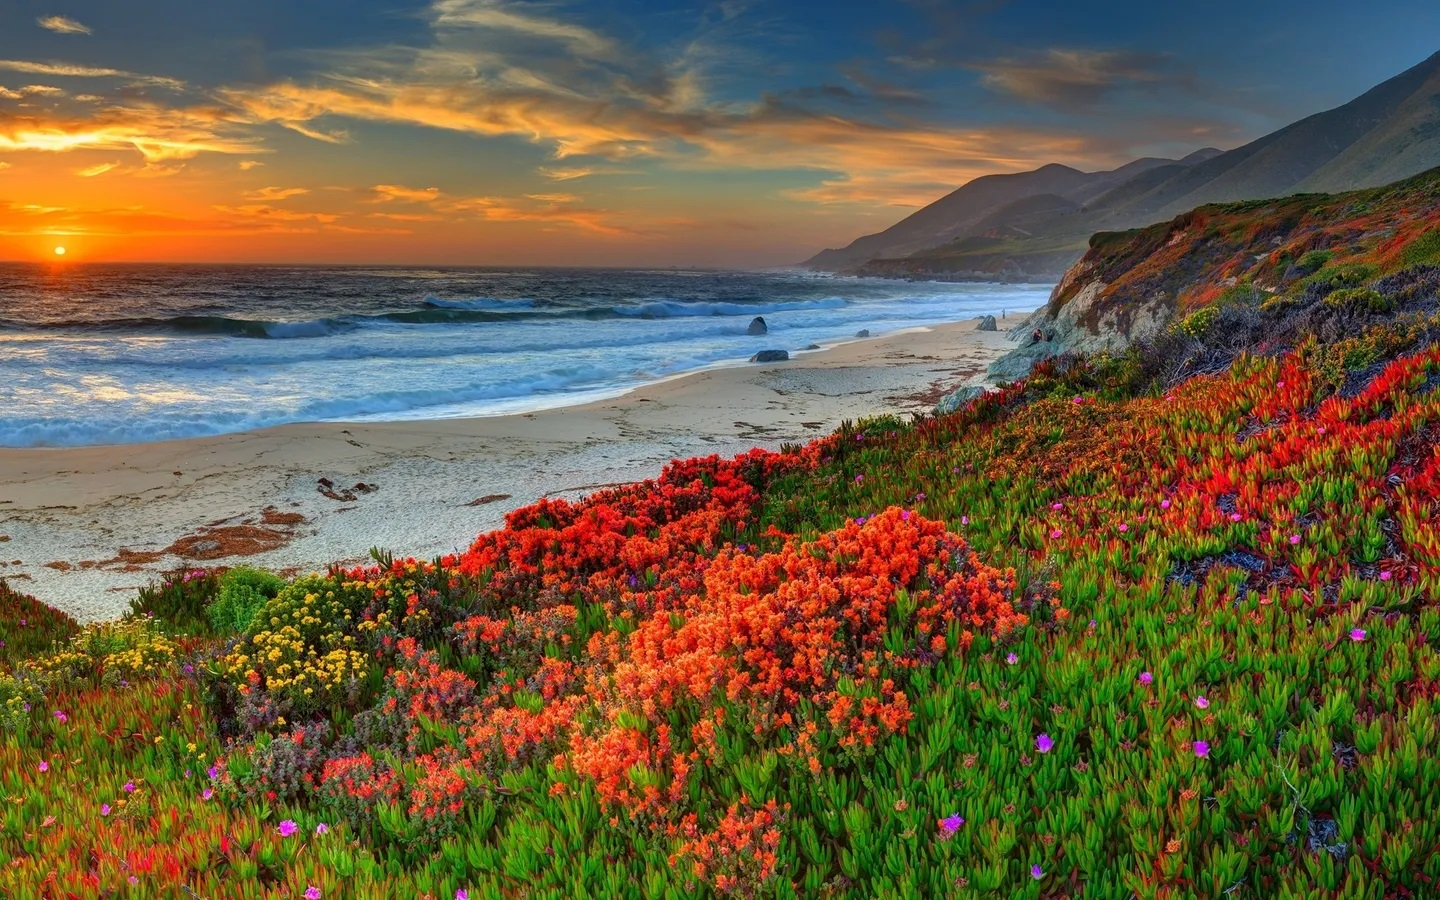
\includegraphics[width=0.9\textwidth]{figures/test.jpg}
    \caption{这里插入了一个普通的相片}
    \label{fig:my_pic1}
\end{figure}
\subsection{多图插图方法}
多图插图方法主要是用到subfigure来进行插图处理。
\begin{figure}[htbp]
    \centering
    \subfigure[泰山]{
        \begin{minipage}[t]{0.48\linewidth}
            \centering
            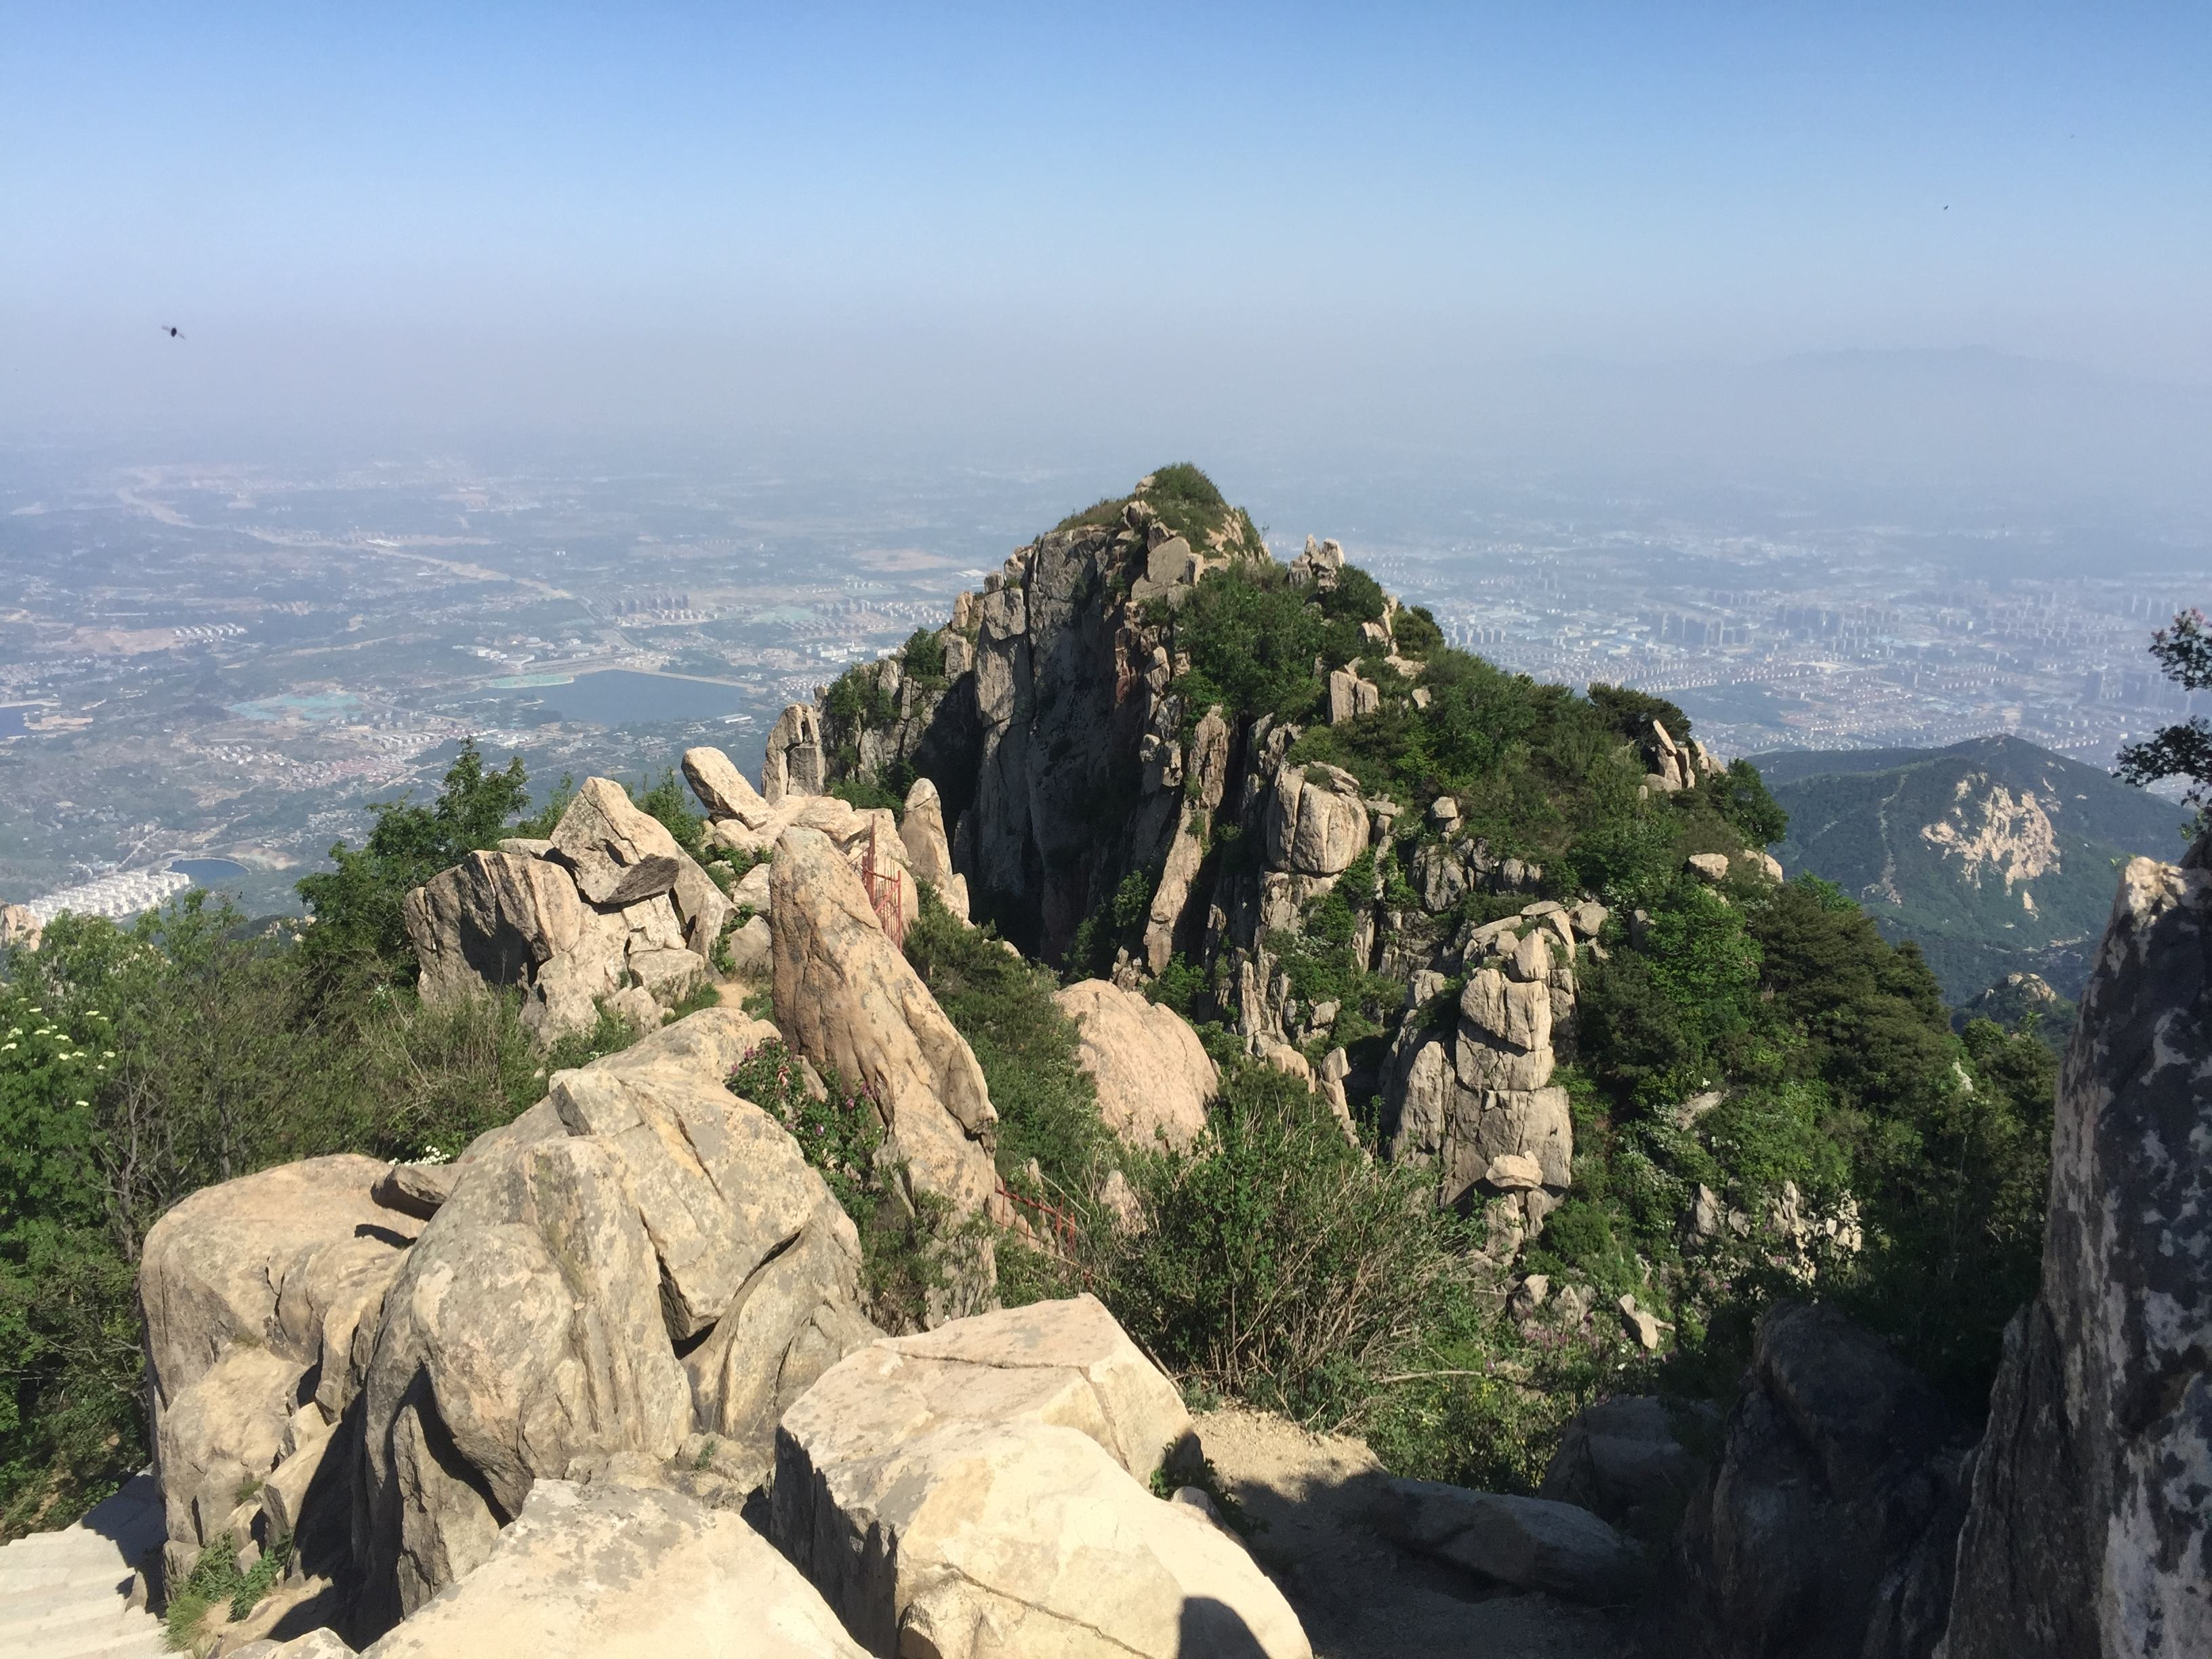
\includegraphics[width=0.9\linewidth]{figures/taishan.jpeg}
        \end{minipage}
    }
    \subfigure[桂林山水]{
        \begin{minipage}[t]{0.48\linewidth}
            \centering
            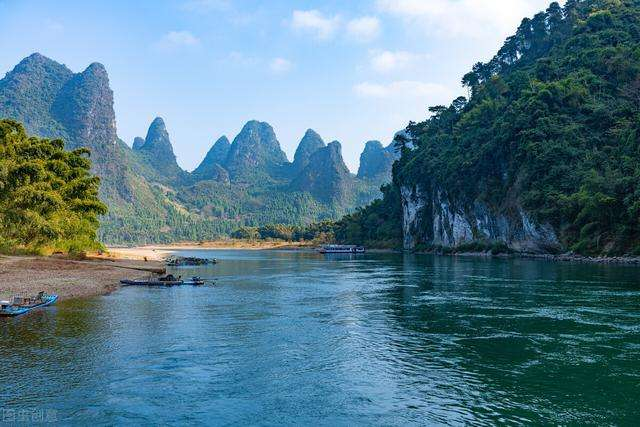
\includegraphics[width=0.9\linewidth]{figures/guilin.jpeg}
        \end{minipage}
    }
    \subfigure[锡林郭勒盟草原]{
        \begin{minipage}[t]{0.48\linewidth}
            \centering
            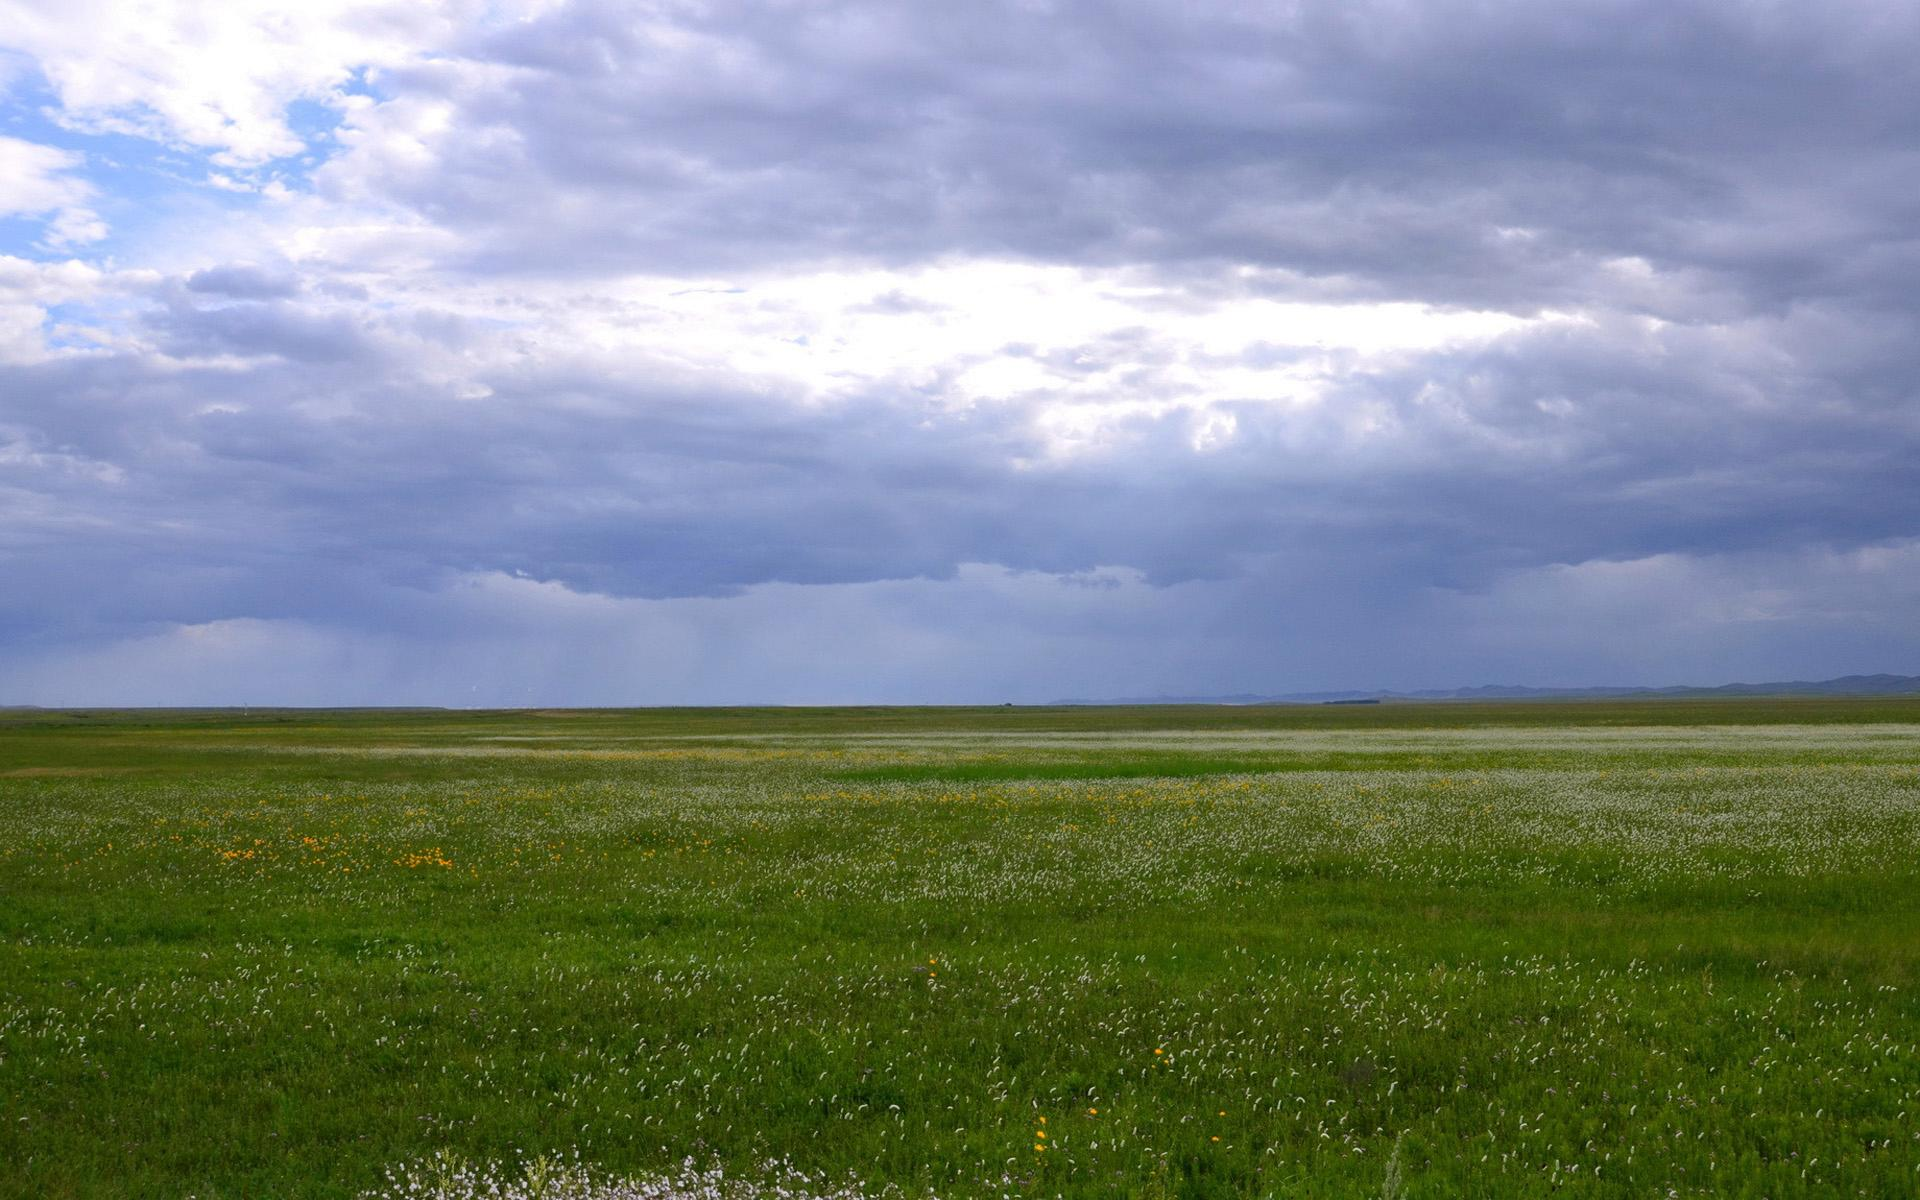
\includegraphics[width=0.9\linewidth]{figures/xilinguole.jpeg}
        \end{minipage}
    }
    \subfigure[布达拉宫]{
        \begin{minipage}[t]{0.48\linewidth}
            \centering
            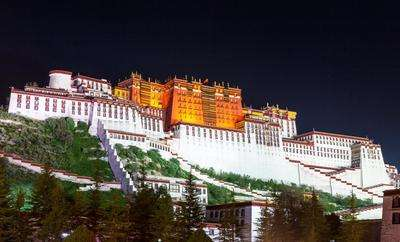
\includegraphics[width=0.9\linewidth]{figures/budalagong.jpeg}
        \end{minipage}
    }
    \centering
    \caption{示例的四张风景图片}
\end{figure}

\subsection{latex自带的一些插图方法}

另外一种就是latex自带的一种画图方法,这里示例两种latex自带的画图方法。
\begin{enumerate}
    \item \textbf{复杂网络结构图}:如图\ref{fig:complex_fig}(a) 所示。
    \item \textbf{函数图像}:如图\ref{fig:complex_fig}(b),(c) 所示,详细参考\href{https://pgfplots.sourceforge.net/gallery.html},函数图像的画法使用到的是pgfplots库当中的元素画图。
\end{enumerate}

\begin{figure}
    \centering
    \caption{latex自带工具画图}
    \label{fig:complex_fig}
    \subfigure[复杂网络结构图]{
        \begin{minipage}[t]{0.9\linewidth}
            \centering
            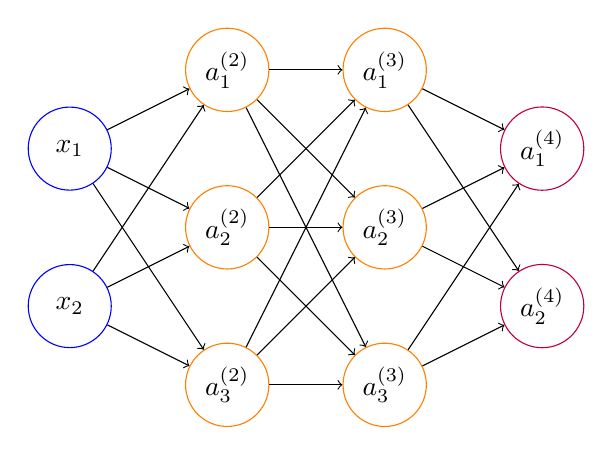
\begin{tikzpicture}
                \node[circle,
                    minimum width =30pt ,
                    minimum height =30pt ,draw=blue] (1) at(0,2){$x_1$};
                \node[circle,
                    minimum width =30pt ,
                    minimum height =30pt ,draw=blue] (2) at(0,0){$x_2$};
                \node[circle,
                    minimum width =30pt ,
                    minimum height =30pt ,draw=orange] (3) at(2,-1){$a_3^{(2)}$};
                \node[circle,
                    minimum width =30pt ,
                    minimum height =30pt ,draw=orange] (4) at(2,1){$a_2^{(2)}$};
                \node[circle,
                    minimum width =30pt ,
                    minimum height =30pt ,draw=orange] (5) at(2,3){$a_1^{(2)}$};
                \node[circle,
                    minimum width =30pt ,
                    minimum height =30pt ,draw=orange] (6) at(4,-1){$a_3^{(3)}$};
                \node[circle,
                    minimum width =30pt ,
                    minimum height =30pt ,draw=orange] (7) at(4,1){$a_2^{(3)}$};
                \node[circle,
                    minimum width =30pt ,
                    minimum height =30pt ,draw=orange] (8) at(4,3){$a_1^{(3)}$};
                \node[circle,
                    minimum width =30pt ,
                    minimum height =30pt ,draw=purple] (9) at(6,2){$a_1^{(4)}$};
                \node[circle,
                    minimum width =30pt ,
                    minimum height =30pt ,draw=purple] (10) at(6,0){$a_2^{(4)}$};
                \draw[->] (1) --(3);
                \draw[->] (1) --(4);
                \draw[->] (1) --(5);
                \draw[->] (2) --(3);
                \draw[->] (2) --(4);
                \draw[->] (2) --(5);
                \draw[->] (3) --(6);
                \draw[->] (3) --(7);
                \draw[->] (3) --(8);
                \draw[->] (4) --(6);
                \draw[->] (4) --(7);
                \draw[->] (4) --(8);
                \draw[->] (5) --(6);
                \draw[->] (5) --(7);
                \draw[->] (5) --(8);
                \draw[->] (6) --(9);
                \draw[->] (6) --(10);
                \draw[->] (7) --(9);
                \draw[->] (7) --(10);
                \draw[->] (8) --(9);
                \draw[->] (8) --(10);
            \end{tikzpicture}
        \end{minipage}
    }
    \subfigure[函数图像]{
        \begin{minipage}[t]{0.4\linewidth}
            \centering
            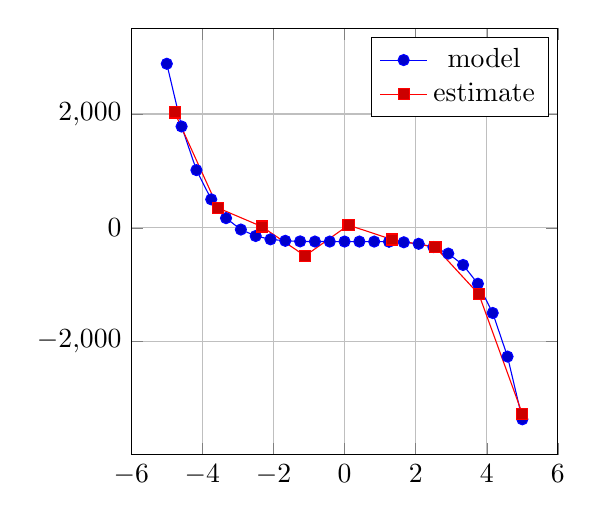
\begin{tikzpicture}
                \begin{axis}[
                    height=7cm,
                    width=7cm,
                    grid=major,
                ]
                    
                \addplot {-x^5 - 242};
                \addlegendentry{model}
            
                \addplot coordinates {
                    (-4.77778,2027.60977)
                    (-3.55556,347.84069)
                    (-2.33333,22.58953)
                    (-1.11111,-493.50066)
                    (0.11111,46.66082)
                    (1.33333,-205.56286)
                    (2.55556,-341.40638)
                    (3.77778,-1169.24780)
                    (5.00000,-3269.56775)
                };
                \addlegendentry{estimate}
                \end{axis}
            \end{tikzpicture}
        \end{minipage}
    }
    \quad
    \subfigure[统计图]{
        \begin{minipage}[t]{0.4\linewidth}
            \centering
            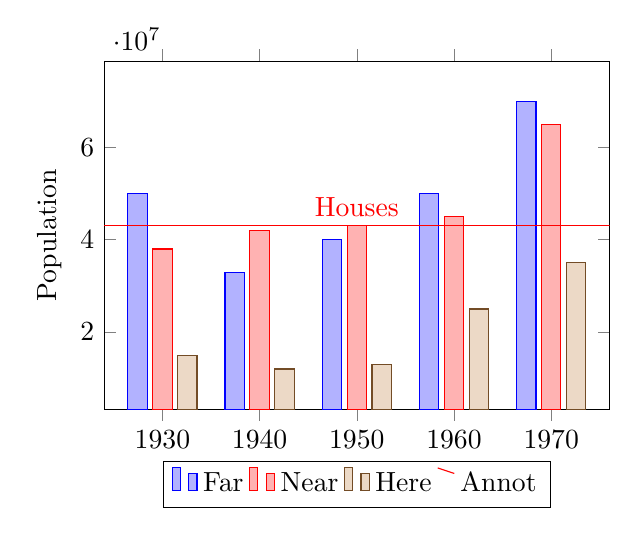
\begin{tikzpicture}
                \begin{axis}[
                    height=6cm,
                    width=8cm,
                    x tick label style={
                        /pgf/number format/1000 sep=},
                    ylabel=Population,
                    enlargelimits=0.15,
                    legend style={at={(0.5,-0.15)},
                        anchor=north,legend columns=-1},
                    ybar,
                    bar width=7pt,
                ]
                \addplot 
                    coordinates {(1930,50e6) (1940,33e6)
                         (1950,40e6) (1960,50e6) (1970,70e6)};
                
                \addplot 
                    coordinates {(1930,38e6) (1940,42e6) 
                        (1950,43e6) (1960,45e6) (1970,65e6)};
                
                \addplot 
                    coordinates {(1930,15e6) (1940,12e6) 
                        (1950,13e6) (1960,25e6) (1970,35e6)};
                
                \addplot[red,sharp plot,update limits=false] 
                    coordinates {(1910,4.3e7) (1990,4.3e7)} 
                    node[above] at (axis cs:1950,4.3e7) {Houses};
                
                \legend{Far,Near,Here,Annot}
                \end{axis}
            \end{tikzpicture}
        \end{minipage}
    }
\end{figure}

\newpage
\subsection{举例表格画法}
表\ref{tab:some_products_datasets}所示是一个简单的双并排表的一个画法。
\begin{table}[htp!]
    \centering
    \caption{某行业产量与生产费用的数据}
    \label{tab:some_products_datasets}
    \newcolumntype{Y}{>{\centering\arraybackslash}X}
    \newcolumntype{Z}{!{\vline}@{\color{white}\vrule width \doublerulesep}!{\vrule}}%自定义列格式(双线)
    \begin{tabularx}{0.94\textwidth}{c|c|YZc|c|Y}
        \Xhline{0.9pt}
        企业编号&	产量(台)&生产费用(万元)&企业编号&产量(台)&生产费用(万元)\\
        \Xcline{1-3}{0.6pt}\Xcline{4-6}{0.6pt}
        1&	40&	130&7&	84&	165\\
        2&	42&	150&8&	100&	170\\
        3&	50&	155&9&	116&	167\\
        4&	55&	140&10&	125&	180\\
        5&	65&	150&11&	130&	175\\
        6&	78&	154&12&	140&	185\\
        \Xhline{0.72pt}
    \end{tabularx}
\end{table}

当然也可以画一个较为复杂的表,如表\ref{tab:model_dataset}所示

\begin{table}[hbpt]
    \centering
    \caption{一个数据表例子}
    \label{tab:model_dataset}
    \begin{tabular}{c|p{1cm}<{\centering}p{1cm}<{\centering}p{1cm}<{\centering}p{1cm}<{\centering}p{1cm}<{\centering}p{1cm}<{\centering}p{2cm}<{\centering}}
        \Xhline{2pt}
        Train & ND & YOS & LIB & YOS & LIB & ND & \multirow{2}{*}{Mean} \\
        \cmidrule(r){0-1}\cmidrule(lr){2-3}\cmidrule(lr){4-5}\cmidrule(lr){6-7}
        Test & \multicolumn{2}{c}{LIB} & \multicolumn{2}{c}{ND} & \multicolumn{2}{c}{YOS} &\\
        \Xcline{1-1}{0.4pt}
        \Xhline{1pt}
        
        SIFT [23] & \multicolumn{2}{c}{29.84} & \multicolumn{2}{c}{22.53} & \multicolumn{2}{c}{27.29} & 26.55\\
        TFeat [3] & 7.39 & 10.13 & 3.06 & 3.80 & 8.06 & 7.24 & 6.64 \\
        L2-Net [46] & 2.36 & 4.70 & 0.72 & 1.29 & 2.57 & 1.71 & 2.23 \\
        HardNet [26] & 1.49 & 2.51 & 0.53 & 0.78 & 1.96 & 1.84 & 1.51 \\
        DOAP [15] & 1.54 & 2.62 & 0.43 & 0.87 & 2.00 & 1.21 & 1.45 \\
        SOSNet [47] & 1.08 & 2.12 & 0.35 & 0.67 & 1.03 & \textbf{0.95} & 1.03 \\
        \textbf{HyNet} & \textbf{0.89} & \textbf{1.37} & \textbf{0.34} & \textbf{0.61} & \textbf{0.88} & 0.96 & \textbf{0.84} \\
        \Xhline{2pt}
    \end{tabular} 
\end{table}


